\input{/Users/daniel/github/config/preamble-por.sty}%available at github.com/danimalabares/config
%\input{/Users/daniel/github/config/thms-por.sty}%available at github.com/danimalabares/config

\newcommand{\rightlooparrow}{\mathbin{
    \vbox{\openup-10.25pt\halign{\hss$##$\hss\cr\circ\cr\longrightarrow\cr}}
}}

\begin{document}
\bibliographystyle{alpha}

\begin{minipage}{\textwidth}
	\begin{minipage}{1\textwidth}
		\hfill Daniel González Casanova Azuela
		
		{\small Prof. Luis Florit\hfill\href{https://github.com/danimalabares/rg}{github.com/danimalabares/rg}}
	\end{minipage}
\end{minipage}\vspace{.2cm}\hrule

\vspace{10pt}
{\huge Geometria Riemanniana}
\tableofcontents
\section{Aula 1}

\subsection{Lembrando}

\begin{defn}\leavevmode
\textit{\textbf{Variedade diferenciável}}
\begin{enumerate}
\item \(M\) espaço topológico Hausdorff (\(T^2\)), base enumerável. Essas duas condições são equivalentes à existência de partições da unidade.

\item \(M\) localmente euclídeo, i.e. \(\mathcal{A}=\{(\chi_\lambda,U_\lambda)\}\), \(\chi_\lambda:U_\lambda \subset M \to\chi_\lambda(U_\lambda)\subset \mathbb{R}^n\), com \(M=\bigcup_{\lambda}U_\lambda\). Dizemos que \(n\) é a \textit{\textbf{dimensão}} de \(M\).

\item Restringindo dois abertos \(U_\lambda\), \(U_\mu\) com \(U_\lambda \cap U_\mu \neq  \varnothing\), a \textit{\textbf{mudança de coordenadas}} \(\chi_\mu \circ \chi_\lambda^{-1}:\chi_\lambda(U_\lambda \cap U_\mu) \to \chi_\mu(U_\lambda \cap U_\mu)\) deve ser diferenciável. (Nesse curso diferenciável é \(C^\infty\) a menos que especifiquemos).

\item Maximalidade, i.e. \(\mathcal{A}\) é maximal.
\end{enumerate}
\end{defn}

\begin{defn}[Mapa diferenciável]\leavevmode
\(f:M^n \to N^m\) se para todo ponto com cartas \((x,U)\) de  \(M\) e \((y,V)\) de \(N\) o mapa \(y \circ f \circ x^{-1}\) é diferenciável. Denotaremos o conjunto de funções diferenciaveis por \(\mathcal{F}(M,N)\). Em particular \(\mathcal{F}(M):=\mathcal{F}(M,\mathbb{R})\).

\end{defn}

\begin{defn}[Espaço tangente]\leavevmode
\(\mathcal{F}_p(M)\) é o espaço de funções definidas num aberto de \(p\) identificando duas delas se coincidem em qualquer aberto contendo \(p\).

\[T_pM:=\{v \in \mathcal{F}_p(M)^*:v(fg)=f(p)v(g)+g(p)v(f)\}\]
\end{defn}

\begin{question}\leavevmode
\(\mathcal{F}_p(M)\) es el stalk de la gavilla de funciones suaves? Qué pasa si definimos algo como las derivaciones en \(\mathcal{F}(U)\).

A la hora de definir base de \(T_pM\) con los operadores \(\partial_i\) necesitamos fijar una carta, así que en realidad no hay una base canónica de \(T_pM\).
\end{question}

\begin{defn}[Diferencial de uma função]\leavevmode
\[df_p:T_pM \to T_{f(p)}N\]
definida para \(g \in T_{f(p)}N\) como
\[df_p(v)(g)=v(g \circ f)\]
\end{defn}

\begin{remark}\leavevmode
A regra da cadeia é uma tautologia dessa definição!
\end{remark}

\begin{defn}[Base canônica do espaço tangente]\leavevmode
Definimos
\[\partial_i |_{p}=\frac{\partial }{\partial x_i}\Big|_{p}\in T_pM\]
como, para \(g \in T_pM\),
\[\frac{\partial }{\partial x_i}\Big|_{p}(g)=\frac{\partial (g \circ x^{-1})}{\partial u_i}\]
\end{defn}
\begin{exercise}\leavevmode
Mostre que \(\{\partial_1|_{p},\ldots, \partial_n|_{p}\}\) é uma base de \(T_pM\).
\end{exercise}

\begin{proof}[Solution]\leavevmode
Primeiro note que \(\{\partial_i|_{p}\}\) é linearmente independente. Suponha que 
\[\sum a_i \partial_i|_{p} =0\]
Then for every function this gives zero, so in particular for coordinate functions \(x_i:U \to \mathbb{R}\), so
\[0=\Big(\sum a_i \partial_i\Big)x_j=\sum a_i \delta_{ij}=a_j\qquad \text{for all \(j\).} \]
Now let's check \(\operatorname{span}\partial_i|_{p}=T_pM\). Choose a vector \(v \in T_pM\) and let
\[w:=v-\sum_{i}v(x_i)\partial_i|_{p}.\]
We wish to show that \(w=0\).

Then there's the following trick: a function \(g:\mathbb{R} \to \mathbb{R}\) with \(g(0)=0\) can be written \(g(t)=th(t)\) for some continuous function \(h\) (subexercise: construct \(h\), it's an integral). So if we define \(\tilde{g}(t)=g(t)-g(0)\) we can write for any \(g: \mathbb{R} \to \mathbb{R}\) (without asking that \(g(0)=0\)) just \(g(t)=g(0)+th(t)\)

\begin{thing6}{Subexercise}\leavevmode
Mostre que para toda \(g:\mathbb{R} \to \mathbb{R}\) existe \(h: \mathbb{R} \to \mathbb{R}\) contínua tal que \(g(t)=g(0)-th(t)\). \textbf{Solution.} Let \(m_x:\mathbb{R} \to \mathbb{R}\) be the function that multiplies \(t\) times a fixed number \(x\). Notice that, for a fixed \(x\), by fundamental theorem of Calculus
\[\int_0^1\frac{d}{dt}(g \circ m_x)(t)dt=g(x)-g(0)\]
and also
\[\int_0^1\frac{d}{dt}(g \circ m_x)(t)dt=\int_0^1 g'(xt)\cdot x=x \int_0^1 g'(xt)dt\]
Then we define
\[h(x):=\int_0^1g'(xt)dt\]
and immediately we get \(g(x)=g(0)-xh(x)\).
\end{thing6}
\begin{thing6}{Subsubexercise}\leavevmode
	Now do that for \(g:\mathbb{R}^n\to \mathbb{R}\). I think the correct claim is that there exists \(h:\mathbb{R}^n\to \mathbb{R}^n\) such that for every \(\vec{x} \in \mathbb{R}^n\) we have \(g(\vec{x})=g(\vec{0})+\vec{x}\cdot h(\vec{x})\). \textbf{Solution.} Now \(m_x\) multiplies the vector \(x\) times the real number \(t\), it is a function \(m_x: \mathbb{R}\to \mathbb{R}^n\). We get
\[\int_0^1 \frac{d}{dt}(g \circ m_x)(t)dt=g(\vec{x})-g(\vec{0}).\]
And also
\[\int_0^1 \frac{d}{dt}(g \circ m_x)(t)dt=\int_0^1 \nabla_{t \vec{x}} g\cdot \vec{x} dt=\int_0^1 \sum \frac{\partial }{\partial x_i}g\Big|_{t\vec{x}}x_i dt=\sum x_i \cdot  \int_0^1 \frac{\partial g}{\partial x_i}\Big|_{t \vec{x}}.\]
Definimos
\[h(\vec{x}):=\left(\int_0^1 \frac{\partial g}{\partial x_1}\Big|_{t \vec{x}}dt, \ldots , \int_0^1 \frac{\partial g}{\partial x_n}\Big|_{t \vec{x}}dt\right) \]
\end{thing6}

{\color{6}\bfseries Back to the original exercise…}\hspace{.5em}Let's try to use this trick to conclude that \(w(g)=0\) for all \(g \in \mathcal{F}_p\). Since it's a local statement I just suppose that \(g\) is a function  \(g: \mathbb{R}^n \to \mathbb{R}\). Then there is a function \(h:\mathbb{R}^n \to \mathbb{R}^n\) such that for every \(x \in \mathbb{R}^n\), \(g(x)=g(0)+x\cdot h(x)\).

Right so remember that I chose an arbitrary vector \(v \in T_pM\) and defined \(w=v-\sum v(x_i)\partial_i|_{p}\). I can see that \(w(x_i)=0\) for all coordinate functions \(x_i\). But also for \(g\) as above I get
\begin{align*}
w(g)&=w(g(0)+x\cdot h(x))=w(x \cdot  h(x))=w\left(\sum x_i h_i(x)\right) =\sum w(x_i h_i(x))\\
&=\sum \cancelto{0}{w(x_i)}h_i(x)+x_ih_i(x)
\end{align*}
and the second term also vanishes if we suppose that the coordinates of our point, \(x_i\), are all zero. {\color{2}Which makes me think: I think that's the point of the trick, that it somehow manages to put the coordinates of the point inside the whole thing, and then we can suppose the coordinates are 0 and simplify everything}.
\end{proof}

\begin{defn}[Fibrado tangente]\leavevmode
Como os \(\mathcal{F}_p(M)\) são disjuntos, porque \(M\) é Hausdorff, os espaços tangentes são disjuntos para pontos distintos.
\[TM:=\bigsqcup_{p \in M}T_pM\]
com a estrutura diferenciável que você já conhece.

A projeção natural \(\pi:TM \to M\) é uma sumersão no sentido da seguinte definição. (Exercício?)
\end{defn}

\begin{defn}[Imersão e sumersão]\leavevmode
\begin{enumerate}
\item Imersão se para todo \(p \in M\), \(df_p\) é injetiva (e isso implica que \(n \leq  m\)).
\item \textit{\textbf{Sumersão}} de \(df_p\) é sobrejetiva para todo \(p\), implicaq ue \( n \geq  m\).
\item \textit{\textbf{Difeomorfismo local}} se para todo ponto \(df_p\) é um isomorfismo. Isso é equivalente a que para todo ponto existe um aberto tal que \(f|_{U}:U \to V\) é um difemorfismo (teo. função inversa). (Checar.)
\end{enumerate}
\end{defn}

Note que \(f: M \to N\) contínua é como dizer que a topologia induzida por \(f\), \(\tau_f \subset \tau_M\). Mas a igualdade nem sempre tem (e.g. figura 8). \(f\) é um \textit{\textbf{mergulho }} se \(\tau_f = \tau_M\). Isso é equivalente a que \(f(M) \subset N\) seja uma subvariedade e \(f:M \overset{\operatorname{difeo}}{\simeq}f(M)\subset N\).

\begin{defn}[Campo coordenado]\leavevmode
Numa vizinhança \(U\) de \(p\),
\begin{align*}
	\partial : U &\longrightarrow TU\subset TM \\
	p &\longmapsto \frac{\partial }{\partial x_i}\Big|_{p}\in T_pM
\end{align*}
\end{defn}

\begin{remark}\leavevmode
Podemos quase extender esse campo. Num aberto \(V \subset U\) cujo fecho \(\bar{V} \subset U\). Pega a coberta \(\{ M \setminus \bar{V}, U\}\). Então existe part. unidade  \((\xi,\varphi)\). Por definição, \(\varphi|_{V} =1\). Defina \(x= \varphi \partial_i\).
\end{remark}

\begin{defn}[Fibrado vetorial]\leavevmode
Um \textit{\textbf{fibrado vetorial }} \(E^k\) sobre \(M^n\) de posto \(k \in \mathbb{N} \cup  \{0\}\) é
\begin{enumerate}
\item \(\pi:E \to M^n\) submersão sobrejetiva.
\item \(\forall  p \in M\), \(E_p = \pi^{-1}(p)\) é um \(\mathbb{R}\)-e.v. de dimensão \(k\).
\item \(\forall p \in M\), existe \(p \in U \subset M\) y \(\varphi_U\) tal que
	\begin{enumerate}
\item  \(\varphi_U: \pi^{-1}(U) \overset{\operatorname{dif}}{\simeq}U \times \mathbb{R}^k\).
\item \(\varphi_U\) conmuta con la proyección, i.e.
	\[\begin{tikzcd}
	\pi^{-1}(U)\arrow[r,"\varphi_U"]\arrow[d,"\pi",swap]&U \times \mathbb{R}^k\arrow[dl,"\pi_1"]\\
	U
	\end{tikzcd}\]
	\item \(\forall  q \in U\), \(\varphi|_{E_q}:E_q \to \{q\} \times \mathbb{R}^k\cong\mathbb{R}^k\) é um isomorfismo linear.
		\end{enumerate}

	Isso é equivalente a pedir que exista um \textit{\textbf{atlas trivializante}} de \(E\). É \(\{(\varphi,\underbrace{\pi(U)}_{\subseteq E}:U \in \Lambda \subset \tau_M\}\) es decir una familia de abiertos en \(E\) indexada por una familia de abiertos de \(M\). Considere dos de estos abiertos con \(W:=U \cap V \neq  \varnothing\).
	\[\begin{tikzcd}
		\varphi_U|_{\pi(W)}\pi^{-1}(W)\arrow[r]& W \times \mathbb{R}^k\arrow[d]\\
		\varphi_V|_{\pi^{-1}(W)}\pi^{-1}(W)\arrow[r]&W \subset \mathbb{R}^k
	\end{tikzcd}\]
onde estamos parametrizando numa variedade! Ou seja, implícitamente estamos pegando cartas nela, mas podemos deixá-lo assim.

Temos as funções de transição
\[\varphi_{VU}=\varphi_V \circ \varphi_U^{-1}|_{W\times\mathbb{R}^k}:W\times\mathbb{R}^k \to W \times \mathbb{R}^k\]
que realmente estão determinadas por a parte linear:
\[\varphi_{VU}(Q,v)=(Q,\xi_{VU}(Q)(v)\]
onde
\[\xi_{VU}:W \to \mathsf{GL}(k,\mathbb{R})\]
e são chamadas de \textit{\textbf{funções de transição}} de \(E\). Elas satisfacem
\[\xi_{VU}\circ\xi_{SV}=\xi_{SU}\qquad \text{cocycle condition} \]
\[\text{no seria…} \qquad \xi_{VU}\circ\xi_{US}=\xi_{VS}\]
Então podemos formar um fibrado vetorial a partir das funções de transição só.
\end{enumerate}
\end{defn}

\section{Aula 2}

\subsection{Fibrados vetoriais}

\begin{defn}\leavevmode
Um \textit{\textbf{fibrado vetorial}} é uma submersão sobrejetora
\[\pi:E \to M\]
onde \(\pi\) é a \textit{\textbf{projeção}},  \(E\) o \textit{\textbf{espaço total}} e \(M\) a \textit{\textbf{base}}. Satisfazendo
\begin{enumerate}
\item \(E\) possui um \textit{\textbf{atlas trivializante}}, i.e. para todo \(p \in M\) existe \(U \ni p\) aberto e carta
		\[\varphi: \pi^{-1}(U) \overset{\operatorname{difeo}}{\to} U \times \mathbb{R}^k\]
		tal que
	\begin{itemize}
	\item \(\pi \circ \varphi_U = \pi|_{\pi^{-1}(U)}\) 
	\item Se \(W=U \cap V \neq  \varnothing\), 
		\begin{align*}
			\varphi_V \circ \varphi_U^{-1} |_{W \times \mathbb{R}^k}: W \times \mathbb{R}^k &\longrightarrow W \times \mathbb{R}^k \\
			(p,v) &\longmapsto (p,\xi_W(p)(v))
		\end{align*}
	onde pedimos que \(\xi_{VU}:W \to \mathsf{GL}(k,\mathbb{R})\), e chamamos esas funções de \textit{\textbf{funções de transição}} de \(E\).
	\end{itemize}
\end{enumerate}
\end{defn}
Note que as fibras são espaços vetoriais: para \(Q \in U\), \(E_Q\overset{\operatorname{def}}{=}\pi^{-1}(Q) \subset E\). Pegue dois elementos \(x, y \in E_Q\). Definimos a soma deles a traves de
\[\varphi(x+y)=(Q,\bar{\varphi} (x)+\bar{\varphi} (y))=(Q,\bar{\varphi} (x+y))\]
onde \(\bar{\varphi} \) é a parte ``linear". Note que isso faz automaticamente que as trivializações sejam lineares nas fibras, i.e. \(E_p \to \{p\}\times \mathbb{R}^k\) linear.

\begin{defn}\leavevmode
As \textit{\textbf{seções de \(E\)}} são
\[\Gamma(E)= \left\{ \begin{tikzcd}\lambda:M\arrow[r]\arrow[rd,"\operatorname{id}"]&  E \arrow[d]\\& M\end{tikzcd} \right\} \]
\end{defn}
\begin{question}\leavevmode
Existe uma coleção de \(k\) seções que são uma base de \(T_pM\) em cada ponto? Não.
\end{question}
\begin{remark}\leavevmode
Existe uma base de seções iff \(E \cong M \times \mathbb{R}^k\). Mas isso ainda nem tem sentido…
\end{remark}

\begin{defn}\leavevmode
Um \textit{\textbf{mapa de fibrados}} é
\[\begin{tikzcd}
	F: E\arrow[r]\arrow[d,"\pi"]&  E \arrow[d,"\pi'"]\\
	M \arrow[r,"f"]& M'
\end{tikzcd}\]
que é linear nas fibras, i.e.
 \[F|_{E_Q}: E_Q \to E'_{f(Q)}.\]
 \(F\) é um \textit{\textbf{isomorfismo}} de fibrados vetoriais iff \(F\) é um difeomorfismo e um mapa de fibrados. (Obviamente isso implica que a inversa é um mapa de fibrados.)
\end{defn}
\begin{remark}\leavevmode
Todo fibrado vetorial possui uma base \textit{local} de seções. Porque pego uma base em \(U \times \mathbb{R}^k\) numa trivialização local e pusho ela pra \(\pi^{-1}(U)\).
\end{remark}

\begin{example}[Fibrado dual]\leavevmode
A observação anterior nos da um jeito super simples de construir o fibrado dual: para cada trivializacão local, e para cada ponto definimos a base dual do espaço vetorial original no ponto, e é isso, tudo segue.

Outros exemplos podem ser construidos do mesmo jeito: \(\operatorname{End}(E)\), \(\Lambda^{r}(\mathbb{V})\). A ideia e que ``a álgebra linear pode ser fibralizada por causa de que temos bases locais".
\end{example}

\begin{example}\leavevmode

Outro exemplo, embora não é um fibrado vetorial, é o conjunto de orientações de \(\mathbb{V}\), \(\mathcal{O}(\mathbb{V} ):=\{\text{bases de \(\mathbb{V}\)} \}\Big/ \sim\). Definimos um  \textit{\textbf{fibrado orientável}} se \(\mathcal{O}(E)\) tem uma seção global. Isso se traduz a que em cada ponto exista uma carta tal que a orientaçao.. seja compatível?

Também podemos definir \(M\) \textit{\textbf{orientável}} se \(TM\) orientavel \textit{como fibrado}. \(TM\) sempre é orientavel \textit{como variedade}  porque \(T TM\) é orientável \textit{como fibrado}.
\end{example}

\begin{example}[Tensores=aplicações multilineares]\leavevmode
Pega \(\mathbb{V}\) esp. vect e considere os tensores \(\{T: \mathbb{V} \times \ldots \times\mathbb{V} \to \mathbb{R}\}:=\operatorname{Multi}(E)\). As seções disso são \(\mathfrak{X}^r(E)\). No caso do fibrado tangente se denotam \(T \in \mathfrak{X}^r(M)\overset{\operatorname{def}}{=}\Gamma TM\), e se chamam \textit{\textbf{campos tensoriais}}.
\end{example}

\subsubsection{Tensores}

{\color{6}Ver \cite{tud}, prop. 21.11 ``The tensor criterion":} acho que em aula definimos \(\mathfrak{X}^r(M)\) como sendo o conjunto de mapas \(r\)-multilineares \(T:M \to \underbrace{T_pM\times\ldots\times T_pM}_{r\text{ vezes} }\), mas na verdade deveria ser \((T^*M)^r:= \bigotimes_r T^*M\). (Devemos pegar produto tensorial para construir um fibrado vetorial certinho.)

\begin{exercise}\leavevmode
Mostre que os seguintes dois \(\mathcal{F}(M)\)-módulos são isomorfos:
\begin{align*}
	\left\{\begin{aligned}T: M &\longrightarrow (T^*M)^r \\
			p &\longmapsto \underbrace{T(p): (T_pM)^r \longrightarrow \mathbb{R}}_{\text{\(r\)-\(\mathbb{R}\)-multilinear}}
\end{aligned}\qquad \text{suave} \right\}=\Gamma((T^*M)^r)=\{\text{seções suaves de \((T^*M)^r\)} \} 
\end{align*}
\begin{align*}
\left\{ \begin{aligned}
\hat{T}:\mathfrak{X}^r(M) &\longrightarrow\mathcal{F}(M)\\
X_1,\ldots,X_r &  \longmapsto \hat{T}: M \longrightarrow \mathbb{R}
\end{aligned}\qquad \text{\(r\)-\(\mathcal{F}(M)\)-multilinear} \right\} 
\end{align*}
\end{exercise}

\begin{proof}[Solução]\leavevmode
	Defina o primeiro conjunto como \(A\) e o segundo como \(B\). Pegue \(T \in A\) e defina
\begin{align*}
	\begin{aligned}
		\hat{T}:\mathfrak{X}^r(M) &\longrightarrow\mathcal{F}(M)\\
		V_1,\ldots,V_r &  \longmapsto 
		\begin{aligned}[t]
			\hat{T}: M &\longrightarrow \mathbb{R} \\
			p &\longmapsto T(p)(V_{1,p},\ldots,V_{r,p})
		\end{aligned}
	\end{aligned}
\end{align*}

Ao contrário, pegue \(\hat{T} \in B\) e defina
\begin{align*}
\begin{aligned}
	T: M &\longrightarrow  (T^*M)^r\\
	 p&\longmapsto \begin{aligned}
	 	T(p): (T_pM)^r &\longrightarrow \mathbb{R} \\
		(v_1,\ldots,v_r) &\longmapsto \hat{T}(V_1,\ldots,V_r)
	 \end{aligned}
\end{aligned}
\end{align*}
onde \(V_i\) é uma extensão de \(v_i\) usando partição da unidade.

O lance em  \cite{tud} é usar a propriedade universal do tensor product (qualquer mapa \(A\times B \to X\) se factora por um único mapa  \(A \otimes B \to X\)…)  para comprovar a suavidade daquele mapa.
\end{proof}

\begin{upshot}[del ejercicio]\leavevmode
Que es lo mismo pensar en un operador que come campos vectoriales y da funciones, o un campo {\color{6}*covectorial*}, una cosa que en cada punto me da un operador que come vectores.
\end{upshot}

\begin{thing6}{Siguiente cosa}[A dupla personalidade dos campos vetoriais]\leavevmode
Que podemos pensar que los campos vectoriales son derivaciones. \(\hat{X}:\mathcal{F}(M) \to \mathcal{F}(M)\). Sí porque un campo de vectores en un punto puede ser evaluado en una función y da un número, y bueno satisface Leibniz.
\end{thing6}

Va otra construcción:

\(E\), pega \(\Lambda^{r}(E)\), os mapas \(r\)-alternantes de \(E\), que é um fibrado vetorial. As seções dele,  \(\Gamma(\Lambda^{r}E)\). No caso do fibrado tangente, \(\Omega^r(M):= \Lambda^{r}(TM)\). Entonces a ver de nuevo: pega \(\omega \in \Lambda^{r}TM\). En cada punto me da una aplicación \(e\)-multiniear alternante, pero también lo puedo ver como un mapa \(\omega: \mathfrak{X} M\times .. \times \mathfrak{X}M \to \mathcal{F}M\).

\begin{exercise}\leavevmode
\(M^n\) é orientável \(\iff\) \(\Lambda^{n}M\) possui seção nunca nula.
\end{exercise}

\begin{proof}[Desastre]\leavevmode
\((\implies )\) Em cada ponto \(p \in M\) temos uma base orientada \(\{e_i\}\) de \(T_pM\). Essa base me permite expressar qualquer coleção de \(n\) vetores \(v_1,\ldots,v_n \in T_pM\) como uma matriz \((v^i_{j})\). O determinante dessa matriz é uma \(n\)-forma alternante. 

Note que essa função {\color{2}não} está bem definida na classe de equivalência: bases diferentes que estão na mesma orientação podem ter determinantes bem diferentes. Definindo  \(\omega_p(v_1,\ldots,v_n)=\det v^i_j\) eu queria uma seção não nula de \(\Lambda^{n}M\)… e daí mostrar que ela é suave…

\((\impliedby)\) Pegue \(\omega \in \Lambda^{n}TM\), qualquer ponto \(p \in M\) e uma base \(\{v_i\}\subset T_pM\) tal que \(\omega_p(v_i)=1\). Afirmo que \(p \mapsto [\{v_i\}]\in \mathcal{O}(M)\) é uma seção global de \(\mathcal{O}(M)\). {\color{2}Falta bastante…}

\end{proof}

\begin{proof}[Solução]\leavevmode
 (\(\implies\)) It's a local-to-global situation, use partition of unity! É como a construção da métrica Riemanniana: pega um atlas localmente finito \(\{(U_\lambda,x_\lambda)\}\) e uma partição da unidade subordinada \(\{\rho_\lambda\}\). Pega qualquer um desses abertos e defina
 \[\omega_{U_\lambda}:=dx_1^{\lambda} \wedge \ldots \wedge dx_n^{\lambda}\]
Some:
\[\omega:=\sum_\lambda \omega_{U_\lambda}\]
Note que tá errado, isso pode dar zero em algum ponto. Some bem:
\[\omega:=\sum_{\substack{ \lambda\text{ t.q.}  \\ \rho_\lambda>0}}\omega_{U_\lambda}\]

\((\impliedby)\) (Inspirado por \cite{les}.) Pegue \(\omega \in \Lambda^{n}TM\), qualquer ponto \(p \in M\). Como \(\omega\) nunca é zero, não é zero em \(p\), e por linearidade existe uma base \(\{v^p_i\}\subset T_pM\) tal que \(\omega_p(v^p_i)=1\). Defina uma orientação pontual (i.e. uma seção de \(\mathcal{O}(M)\), \textit{não necessariamente contínua} da seguinte forma: uma base qualquer de \(T_pM\) é orientada se está na mesma classe de equivalência que \(\{v^p_i\}\).

Para ver que essa seção de \(\mathcal{O}(M)\) é contínua devemos mostrar (de acordo a \cite{les}) que em cada ponto \(p\in M\) existe um marco local que da uma base orientada em cada ponto. Então pegue uma vizinhança coordenada de qualquer ponto \(p\) e considere a função \(f\) tal que
\[\omega=fdx_1 \wedge \ldots \wedge dx_n\]
Então
\[\omega(\partial_1,\ldots, \partial_n)=f \leftsquigarrow \text{ nunca se anula} \]
Então a base coordenada é sempre positiva ou sempre negativa (em \(U\)). Pode supor que é sempre positiva botando um menos em qualquer função coordenada.  Aí note que \(f\) também é
\[\omega(\partial_1,\ldots,\partial_n)=\underbrace{\det C}_{=f}\omega(v^q_1,\ldots,v^q_n) \qquad  \forall  q \in U\]
Porque é assim o assunto da mudança de base… e aí acabou porque \(f=\det C>0\).

\end{proof}

Lembre que \(\Omega_c^n(M)\) é o espaço de formas cujo suporte tem fecho compacto.

\begin{remark}\leavevmode
\(M\) orientada \(\implies\) integral está bem definida. Sim, porque o teorema de mudança de variáveis diz que para \(\varphi: U \to V\), \(\omega \in \Omega^{n}(V)\), \(\int_U \varphi^*\omega=\text{*sinal!*}\int_V \omega \). Então para que não se faça uma bagunça precisamos que os determinantes das mudanças de coordenadas coincidam.
\end{remark}

\begin{defn}[Fibrado pullback]\leavevmode
\[\begin{tikzcd}
	f^* (E)\arrow[r,"\pi_2"]\arrow[d,"\pi_1",swap]&E\arrow[d,"\pi"]\\
	M\arrow[r,swap,"f"]&N
\end{tikzcd}\]
onde
\[f^*(E)=\{(p,v) \in M \times E: \pi(v)=f(p)\}\]
(Note que botamos o \(p\) em \((p,v)\) para obter que o espaço total de \(f^*(E)\) seja uma coleção \textit{disjunta} de fibras.)
\end{defn}
Essa é uma definição ótima. Note que \(\pi_2\) é um mapa de fibrados que aparece de graça. (Não é um isomorfismo.)

\begin{remark}\leavevmode
O pullback é mágico porque ele leva todas as propriedades de \(E\) como curvatura, conexão, etc.
\end{remark}

\begin{remark}\leavevmode
Se \(f\) é constante obtemos o fibrado trivial.
\end{remark}

\begin{question}\leavevmode
Me queda claro que si \(f\) es constante, la fibra de \(f^*E\) siempre es \((f^*E)_p \cong E_{f(*)}\)…
\end{question}

\begin{remark}\leavevmode
Pega  \(\xi \in\Gamma(f^* E)\). Então temos para \(p \in M\) um elemento \(\xi(p)=(p, \bar{\xi}(p)) \). Então olha
\[\begin{tikzcd}
	\bar{\xi} :M \arrow[r]\arrow[dr,"f"]&  E \arrow[d,"\pi"]\\& N
\end{tikzcd}\]
então essas seções se chamam de \(\mathfrak{X}_f \cong \Gamma(f^*(E))\) \textit{\textbf{seções ao longo de \(f\)}}.
\end{remark}
Entonces el punto es que, por construcción cada sección del pullback me da un elemento en el otro vb y de ahi quiero que la proyección me devuelva \(f\).

Note que para um campo vetorial \(X \in \mathfrak{X}(M)\) temos um campo \(f_*X\) que \textit{não é} um campo vetorial em \(N\). É um campo vetorial com base \(M\) e espaço total  \(f^*TN\). Parecidamente, se \(Y \in \mathfrak{X}(N)\), obtemos um campo sobre \(M\) com valores em \(f^*TN\) mediante \(Y \circ f\).
\begin{defn}\leavevmode
Dos campos \(X \in \mathfrak{X}(M)\) e \(Y \in \mathfrak{X}(N)\) están \textit{\textbf{\(f\)-relacionados}} \(X \overset{f}{\sim}Y\) se \(Y \circ f =f_*X\) donde \(f:M \to N\). Pero pérame porque a mí me habían dicho que no siempre \(f_*X\) está bien definido. Ah, porque aquí \(f_*X\) es un campo \textit{ao longo de \(f\)}; así \textit{siempre} está bien definido. Entonces tiene sentido la definición y el ejercicio:
\end{defn}

\begin{exercise}\leavevmode
	Pegue \(X_i \in \mathfrak{X}(M)\), \(Y_i\in \mathfrak{X}(N)\), \(i=1,2\). Mostre que  \[X_i \overset{f}{\sim}Y_i\implies [X_1,X_2] \overset{f}{\sim}[Y_1,Y_2]\]
\textbf{Hint.} Pensa que um campo é uma coisa que pega uma função e me da uma função.
\end{exercise}

\begin{proof}[Solução]\leavevmode
	Queremos ver que
	\[f_*[X_1,X_2]=[Y_1,Y_2]\circ f \in \mathfrak{X}_f\]
i.e. que esses campos são iguais \textit{como campos vetoriais ao longo de \(f\)}, que é um negócio bem estranho porque, de novo, o espaço base é \(M\) e o espaço total é \(f^* TN\) (que é bem parecido a \(TN\) mas  não é \(TN\)---pode ser incluído eu acho).

E isso é super importante porque esclarece o jeito de proceder que é: pega \(p \in M\) e \(g \in \mathcal{F}(N)\). Beleza então temos
	\begin{align*}
	\Big([Y_1,Y_2]\circ f\Big)_p(g)&=Y_{1,f(p)}\Big(Y_2(g)\Big)-Y_{2,f(p)}\Big(Y_1(g)\Big)\qquad \text{blz} \\
				       &\overset{\operatorname{hip}}{=}f_*X_{1,p}\Big(Y_2(g)\Big)-f_*X_{2,p}\Big(Y_1(g)\Big)\\
&\overset{\operatorname{hip}}{=}f_*X_{1,p}\Big(f_*X_2(g)\Big)-f_*X_{2,p}\Big(f_*X_2(g)\Big)\\
&=f_*[X_1,X_2]_p(g).
	\end{align*}
\end{proof}

\subsection{Grupos de Lie}

\begin{defn}\leavevmode
Um \textit{\textbf{grupo de Lie}} é um grupo \(G\) que é uma variedade diferenciável tal que
\[\cdot :G \times G \to G \qquad \qquad \leavevmode^{-1}:G \to G\]
são diferenciaveis.
\end{defn}

Os grupos de Lie tem um monte de difeomorfismos dados pela multiplicacão a esquerda: \(h \in G \rightsquigarrow L_h:G \to G\), \(L_h(g)=h\cdot g\). Como \(L_{h^{-1}}\circ L_h=\operatorname{Id}\), \(L_h \in \operatorname{Dif}G\).

\begin{exercise}\leavevmode
\(v \in T_eG\), \(X_v(g)=d(L_g)_e(v) \in T_gG\), \(\implies\) \(X_v \in \mathfrak{X}(G)\). \textbf{Note} que vai precisar usar que o produto do grupo é diferenciável.
\end{exercise}

\begin{proof}[Solução]\leavevmode
Basta mostrar que, pegando qualquer vizinhança coordenada de qualquer ponto \(g \in G\), as funções coordenadas de \(X_v\) são diferenciáveis.

Pegue um sistema de coordenadas em  \(g \in G\), digamos \((U,x)\). Como  \(L_g\) é um difeomorfismo, obtemos um sistema de coordenadas \((L_{g^{-1}}(U),x')\) de \(e \in G\). Suponha que \(v=\sum v^i\partial_i\) nessas coordenadas. Então
\begin{align*}
	(d_eL_g)v&=(d_eL_g)\left(\sum v^i\partial_i\right) \\
	&=\sum (v^i \circ L_g)d_eL_g\partial_i
\end{align*}
Então essas funções coordenadas são suaves: para \(h \in G\) temos
\[(v^i \circ L_g)(h)=v^i(gh)\]
que é suave porque é a composição de duas funções suaves, e porque o produto do grupo de Lie é suave.
\end{proof}
E aí fica que uma base \(\{v_i\}\subset T_eG\) nos da uma base global de seções. Em outras palavras, o fibrado tangente de um grupo de Lie é trivial. Isso é rarísimo, uma variedade com fibrado tangente trivial, se chama variedade paralelizável.

\begin{remark}\leavevmode
\(\forall g \in G, X_v \overset{L_g}{\sim}X_v\) para todo \(v \in T_eG\). Acho que é por regra da cadeia. Queremos ver
que em todo ponto \(g \in G\), \[\Big((L_g)_*(X_v)\Big)_h=(X_v)_h\]
então fica que
\begin{align*}
\Big((L_g)_*(X_v)\Big)_h&=\Big((d_{g^{-1}h}L_g)(d_eL_{g^{-1}h})v\Big)_h=\Big(d_e(L_g\circ L_{g^{-1}h})v\Big)_h=\Big(d_eL_{h}v\Big)_h=(X_v)_h
\end{align*}
Mas ainda, se um campo vetorial \(X\) está \(L_g\) relacionado com ele mesmo para todo \(g \in G\) (isso se chama ser \textit{\textbf{invariante à esquerda}}), então ele é um \(X_v\) para algum \(v\). Conta:
\[v:=X_e \implies X_h=(L_{h,*}X)_h=(d_eL_{h}X_e)_h=d_eL_hv.\]
Então ai fica essa equivalência, e ademais, se pegamos \(v,w \in T_eG\) podemos pensar em \(X_v,X_w\), e \textit{definimos} \(X_{[v,w]}:=[X_v,X_w]\). E ai obtemos a \textit{\textbf{álgebra de Lie}} de \(G\), que é \((T_eG,[,]):=\mathfrak{g}\).
\end{remark}

\begin{thing6}{Mais um}\leavevmode
Pegue \(X \in \mathfrak{g}\) e \(\gamma\) curva integral de \(X\) passando por \(e\), i.e. \(\gamma(0)=e\). Prove que
\begin{enumerate}
\item Se \(\varphi_t\) é o fluxo de \(X\) \(\implies\) \(L_g \circ\varphi_t = \varphi_t\circ L_g\), \(\varphi_t = R_{\gamma(t)}\).
\item \(\gamma\) é homomorfismo de grupos \(\mathbb{R} \to G\). Isso permite definir \(\operatorname{exp}^G: \mathfrak{g} \to G\) dada por \(\operatorname{exp}^G(X)=\gamma(1)\). Prove que \(\operatorname{exp}^G(tX)=\gamma(t)\).

\textbf{Hint.} O último implica os outros.
\end{enumerate}
\end{thing6}

\begin{proof}[Solução]\leavevmode
\begin{enumerate}
\item Pegue \(h \in G\). O único que sei de \(\varphi_t\) é que
	\[\frac{d}{dt}\Big|_{t=0}\varphi_t(h)=X_h\]
E quero ver que
\[\varphi_t(gh)=(\varphi_t \circ L_g)(h)\overset{\text{quero} }{=}(L_g \circ \varphi_t)(h)=g\varphi_t(h)=L_g(\varphi_t(h))\]
Então derivo:
\begin{align*}
\frac{d}{dt}\Big|_{t=0}\varphi_t(gh)&=X_{gh}\overset{\operatorname{def}}{=}d_eL_{gh}(X_e)\overset{\substack{\text{chain}  \\ \text{rule}} }{=}d_hL_gd_eL_h(X_e)\overset{\operatorname{def}}{=}d_hL_gX_h=d_hL_g\left(\frac{d}{dt}\Big|_{t=0}\varphi_t(h)\right) 
\end{align*}
de forma que as derivadas das coisas que quero que sejam iguais coincidem. Avaliando em \(t=0\) vemos que as funções devem ser iguais.

A comprovação de que \(\varphi_t=R_{\gamma(t)}\) é análoga: definindo \(X:=X_{X}\) (e é assim porque \(X\in \mathfrak{g}\)), tenho duas funções
\begin{align*}
\begin{aligned}
R_{\gamma(t)}: G &\longrightarrow G \\
	g &\longmapsto g\cdot\gamma(t)
\end{aligned}\qquad \begin{aligned}
\varphi_t: G &\longrightarrow G \\
g &\longmapsto \substack{\text{integro \(X_g\)}\\\text{e avanço \(t\)} }
\end{aligned}
\end{align*}
Derivo:
\begin{align*}
	\frac{d}{dt}\Big|_{t=0}g\cdot \gamma(t)&=\frac{d}{dt}\Big|_{t=0}(L_g \circ \gamma)(t)\overset{\substack{\text{chain}\\\text{rule}}}{=}d_eL_g\cdot \gamma'(0)=X_g=\frac{d}{dt}\Big|_{t=0}\varphi_t(g)
\end{align*}
avaliando em \(t=0\) obtemos a igualdade.

\item  Talvez tô errado mas acho que é o mesmo: queremos ver que
	\[\gamma(t_1+t_2)\overset{\text{quero}}{=}\gamma(t_1)\gamma(t_2)\overset{\operatorname{def}}{=}L_{\gamma(t_1)}\gamma(t_2)\]
então derivo respeito a \(t_2\) 
\begin{align*}
\frac{d}{dt_2}\Big|_{t_2=0}L_{\gamma(t_1)}\gamma(t_2)&\overset{\substack{\text{chain}\\\text{rule}}}{=}d_{\gamma(0)}L_{\gamma(t_1)}\gamma'(0)=d_eL_{\gamma(t_1)}X_e\\&=X_{\gamma(t_1)}\overset{\substack{\text{\(\gamma\) curva}  \\ \text{integral} }}{=} \gamma'(t_1)=\frac{d}{dt_2}\Big|_{t_2=0}\gamma(t_1+t_2)
\end{align*}
e de novo, avaliando em \(t_2=0\) obtemos a igualdade.

Por fim, para o último exercício queremos achar uma curva integral de \(tX\), \(t\) fixo, i.e.
\[\tilde{\gamma}:\mathbb{R}\to G\qquad \text{tal que} \qquad \tilde{\gamma}'(s)=(tX)_{\tilde{\gamma(s)}}\forall s \in \mathbb{R}.\]
Sinto no cora que 
\[\tilde{\gamma}(s):=\gamma(ts)\qquad \text{vai dar certo.} \]
Então derivo
\[\frac{d}{ds}\Big|_{s=s}\tilde{\gamma}(s)=\frac{d}{ds}\Big|_{s=s}\gamma(ts)=\gamma'(ts)t=X_{\gamma(t s)}t=(tX)_{\gamma( ts)}=(tX)_{\tilde{\gamma}(s)}\]
olha só
\[\operatorname{exp}^G(tX)=\tilde{\gamma}(1)=\gamma(t).\]

\end{enumerate}
\end{proof}

\section{Aula 3: A primeira aula}

\subsection{Lembrando geometria diferencial de curvas e superfícies}

A história começa com o Gauss em \(1827\).

A geometria de superfícies se faz assim. Pega \(p \in M^2 \subset \mathbb{R}^3\). Pode botar uma métrica canônica usando a inclusão \(i\), i.e.
\begin{align*}
	\left<\cdot,\cdot\right>_p: T_pM^2 \times T_pM^2 &\longrightarrow \mathbb{R} \\
	(v,w) &\longmapsto \left<i_{*,p}v,i_{*,p}w\right>_p
\end{align*}
Também pode só derivar curvas na superfície, obtendo vetores em \(\mathbb{R}^3\), e usando o produto usual de \(\mathbb{R}^3\).

O Gauss definiu o mapa normal \(N(p)\), derivando ele para obter
\[A:=d_p N : T_pM ^2 \to T_pM^2\]
que ressoltou ser um endomorfismo autoadjunto (respeito a aquela métrica que a gente falou). Dai apareceram
\[\operatorname{tr}A=H\qquad \text{curvatura média} \]
\[\det A=K\qquad \text{curvatura Gaussiana} \]
E ai o Gauss descobriu que \(K\) depende s ó da métrica, i.e. \(K=K(\left<\cdot,\cdot\right>)\). A curvatura média não. (E.g. um plano pode ser mergulhado em \(\mathbb{R}^3\) como um cilindro, \(K\) fica igual, enquanto \(H\) muda.)

\subsection{Riemann}

\begin{defn}\leavevmode
Uma \textit{\textbf{variedade Riemanniana}} é uma variedade diferenciável \(M^n\) junto com um tensor
\[\left<\cdot,\cdot\right>: \mathfrak{X}(M) \times \mathfrak{X}(M) \longrightarrow \mathcal{F}(M)\]
simétrico e positivo definido. Isso significa que para cada \(p \in M\) temos uma forma bilinear simétrica positiva definida \(\left<\cdot,\cdot\right>_p:T_pM \times T_pM \longrightarrow \mathbb{R}\).

A variedade é \textit{\textbf{semi-Riemanniana}} se, em lugar de positivo definido, o tensor é não degenerado, i.e. \(\forall v \in T_pM\), se \(\left<v,w\right>_p=0\) \(\forall w \in T_pM\), então \(v =0\). Nesse caso, definimos o \textit{\textbf{índice}} da forma como sendo
\[i(\left<\cdot,\cdot\right>_p:=\operatorname{max}\left\{ \dim \mathbb{L} \overset{\text{sub} }{\subset} T_pM:\left<\cdot,\cdot\right>|_{\mathbb{L}\times\mathbb{L}}<0\right\} \]

Bom pegue um sistema coordenado \((x,U)\). Podemos definir para \(Q \in M\)
\[g_{ij}(Q):=\left<\partial_i(Q),\partial_j(Q)\right> \in \mathcal{F}(U)\]
i.e.
\[(g_{ij})_Q:U \longrightarrow \mathsf{GL}(n,\mathbb{R}) \cap \operatorname{Sym}(n)\]
ou seja, a variedade é Riemanniana quando essas funções são positivas.

Se a variedade é Riemanniana temos uma norma \(\|v\|:=\sqrt{v,v} \). (Se não não.)
\end{defn}

\begin{remark}\leavevmode
A definição de variedade Riemanniana foi dada por Weil nos anos 30.
\end{remark}

\begin{defn}[Isometrias]\leavevmode
\(f:M \to N\). Primeiro note que podemos definir o pullback de qualquer tensor. Para \(f:M \to N\) e \(T\) tensor da forma \(T: \mathfrak{X}(N)\times \mathfrak{X}(N) \longrightarrow \mathcal{F}(N)\), definimos
\[f^*(T)_p(u,v)_p:=T(f(p))(f_*u,f_*v)\]
Note que de graça é simétrico se o tensor em \(N\) é simétrico.

Para ver positivo definido temos que o pullback é positivo definido \(\iff\) \(f\) é um imersão. Prova: considera a norma. A norma de \(f_{*,p}u\) é positiva \(\iff\) \(u \neq 0\). Para asegurar que a preimagem desse vetor também  não é zero precisamos que seja imersão (=diferencial injetiva).

{\color{7}Conclusão:} apenas as imersões podem ser isometrias.

\(f:(N^n,\left<\cdot,\cdot\right>_N)\longrightarrow (M^m,\left<\cdot,\cdot\right>_M)\) é uma \textit{\textbf{imersão isométrica}} se \(\left<\cdot,\cdot\right>_N=f^*\left<\cdot,\cdot\right>_M\).

Uma \textit{\textbf{isometria}} entre variedades Riemannianas é \(f:M^n \to \tilde{M}^n\) difeomorfismo e isometria (como imersão).

Uma \textit{\textbf{isometria local}} é um difeo local e isometria.
\end{defn}

\begin{remark}[Isomorfismos canônicos]\leavevmode
Para qualquer espaço vetorial \(\mathbb{V}\), temos um \textit{isomorfismo canônico} (i.e. não depende de escolha de base) \(\mathbb{V}^n \cong T_p\mathbb{V}^n\) dado por
\[\mathbb{V}^n \ni v \longmapsto \alpha_{p,v}'(0),\qquad  \alpha_{p,v}(t)=p+tv\]

Tem outro isomorfismo canônico: \(M\ni p,M' \ni p'\),
\[T_{(p,p')}(M \times M') \cong T_pM \times T_{p'}M'\]
\[w \longmapsto(\pi_{*,(p,p')}(w),\pi'_{*,(p,p')}(w))\]
onde
\[\begin{tikzcd}
&M\times M'\arrow[dl,"\pi",swap]\arrow[dr,"\pi'"]\\
M&&M'
\end{tikzcd}\]
\begin{exercise}\leavevmode
Mostre que o inverso desse mapa ai é
\[(\pi_{*,(p,p')}(w),\pi'_{*,(p,p')}(w) \longmapsto(i_p)_{* p'}(v') + (i'_{p'})_{* p}(v)\]
com as inclusoes naturais.
\end{exercise}
\begin{proof}[Solução]\leavevmode
 Acho que as definições certinhas das inclusões são assim:
\begin{align*}
\begin{aligned}
i_{p'}: M &\longrightarrow M \times M' \\
q &\longmapsto (q,p')
\end{aligned}\qquad
\begin{aligned}
i'_p: M' &\longrightarrow M \times M' \\
	q' &\longmapsto (p,q')
\end{aligned}
\end{align*}
que tem diferenciais
\begin{align*}
\begin{aligned}
	(i_{p'})_p: T_pM &\longrightarrow T_{(p,p')(M\times M')} \\
	v &\longmapsto ?
\end{aligned}\qquad
\begin{aligned}
	(i_p)_{p'}: T_pM &\longrightarrow T_{(p,p')}(M\times M') \\
	 v'&\longmapsto ?
\end{aligned}
\end{align*}

\textbf{*Intento 1*} Para visualizar melhor como funcionam esses mapas considere pegue coordenadas \((x,x')\) de \(M \times M'\) (o que significa por definição da variedade produto que \(x\) são coordenadas de \(M\) e \(x'\) de \(M'\)). Fica que \( \{\partial_i\}\) é base de \(T_pM\) e \(\{\partial_i'\}\) de \(T_{p'}M\). Então
\[v=\sum v_i\partial_i\xmapsto{(i_{p'})_{*p}} \sum v_i\partial_i+\sum 0\partial_i' \leftrightsquigarrow(v_1,\ldots,v_n,0,\ldots,0)\]
O resultado é bastante claro daí. Mas… não é ponto de tudo isso que o isomorfismo é \textit{independente da escolha de base}…?

\textbf{*Intento 2*} Copiemos a prova de que \(\mathbb{V}^n \cong T_p\mathbb{V}^n\) canonicamente… acho que só escrevendo 
\[v:=\gamma'(0), \qquad \gamma:(-\varepsilon,\varepsilon) \longrightarrow M, \gamma(0)=p\]
Obtemos
\[(di_{p'})_{p}(v)=\frac{d}{dt}\Big|_{t=0}(i_{p'} \circ \gamma)(t)=\frac{d}{dt}\Big|_{t=0}(\gamma(t),p)=(\gamma_*(0),0)\]
definindo analogamente \(\gamma'\) (aqui \('\) não é derivada…) de forma que
\[v+v'=(\gamma_*(0),\gamma'_*(0))\]
é projetado ``canonicamente" (=sem usar bases…) em \(v\) e \(v'\) quando aplicamos \(\pi_{*,(p,p')}(v+v')\) e \(\pi'_{*(p,p')}(v+v')\), respetivamente. (É só escrever igualzinho que acima compondo com a projeção…) E acho que é isso.
\end{proof}
\end{remark}

\begin{thing7}{Cuidado}[Não entendi muito isso aqui]\leavevmode
Nem sempre é certo que \(T(M \times M') \cong \)``\(TM \times TM\)". Porque as funções coordenadas dependem de dois parámetros: \(Z \in \mathfrak{X}(M \times M')\), \(Z=X+X'\),
 \[\sum a_i(p,p')\partial_i|_{p}+\sum_{j}b_j(p,p') \partial_j\]
\end{thing7}

\begin{example}\leavevmode
\begin{enumerate}
\item \(\mathbb{R}^n\) com o produto canônico usando o isomorfismo canônico de \(\mathbb{R}^n \cong T_p \mathbb{R}^n\) acima.

\item (Grupo de Lie.) \(h \in G\), \(L_h\) traslação a esquerda. Usemos as traslações a esquerda para definir uma métrica em \(G\). Pegue qualquer produto interno \(\left<\cdot,\cdot\right>_e\) em \(\mathfrak{g}\). E traslade:
	\begin{align*}
	\left<\cdot,\cdot\right>_h&:=L_h^*\left<\cdot,\cdot\right>_e
	\end{align*}
	i.e.,
	\[\left<v,w\right>_h=\left<dL_{h^{-1}}(v),dL_{h^{-1}}(w)\right>_e\]
\begin{exercise}\leavevmode
\begin{enumerate}
\item Isto define uma métrica Riemanniana em \(G\).
 \item \(\forall  X,Y \in \mathfrak{g}\), \(\left<X,Y\right>=\operatorname{cte}\).
 \item \(\left<\cdot,\cdot\right>\) é \textit{\textbf{invariante a esquerda}}, i.e. \(\forall  h \in G\), \(L_h\) é isometria de \((G,\left<\cdot,\cdot\right>)\).
\begin{remark}\leavevmode
Essa métrica é invariante a \textit{a esquerda}. Nem tem que ser invariante a direita.
\end{remark}
\begin{remark}\leavevmode
Vai ter um exercício de do Carmo dizendo que se \(G\) é compacto vai ter uma métrica bi-invariante, i.e. o promédio.
\end{remark}
\end{enumerate}
	{\color{7}dani:} parece que sempre que temos uma ação homogênea podemos transportar a métrica de \(\mathfrak{g}\) pra todos lados.
\end{exercise}	
\begin{proof}[Solução]\leavevmode
\begin{enumerate}
\item Acho que aqui sale facilzinho porque \(L_h\) é um difeomorfismo, i.e. os espaços tangentes são isomorfos, então temos a propriedade de ser positiva definida.

\item É por definição de campo vetorial gerado por traslações a esquerda.

\item Por definição de isometria… tipo--essa métrica está feita para que as traslações sejam isometrias.
\end{enumerate}
\end{proof}
\item \(M^n \subset \mathbb{R}^{n+p}\) subvariedade regular (=inclusão é um mergulho). Podemos fazer o que Gauss fez:
	\[\left<u,v\right>_p:=\left<i_{*,p}u,i_{*,p}v\right>^{\mathbb{R}^{n+p}}_{\operatorname{can}}\]
\end{enumerate}
\end{example}

\begin{question}\leavevmode
Será que toda variedade Riemanniana admite um mergulho isométrico em algum \(\mathbb{R}^{n+p}\)? Quem é \(p\)?
\end{question}

\begin{thing7}{Nash}\leavevmode
O caso \(C^1\) é fácil, 
\end{thing7}

\begin{question}[dani]\leavevmode
Em topo dif vimos primeiro uma prova de que pode mergulhar qualquer variedade em um \(\mathbb{R}^N\) com \(N\) muito grande. Depois os teoremas de Whitney mostrarem que \(N\) pode ser mais o menos pequeno. Aqui podemos mostrar que o mergulho/imersão existe para \(N\gg\) mais o menos facilmente?
\end{question}

\begin{prop}[Existência de métricas Riemannianas]\leavevmode
Se \(M\) é uma variedade diferenciável, existe uma métrica Riemanniana em \(M\).
\end{prop}

\begin{thing6}{What}\leavevmode
que em toda variedade tem um aberto denso difeomorfo a uma bola.
\end{thing6}

\begin{proof}\leavevmode
Pegue um atlas \(\{(X_\lambda,U_\lambda)\}\) localmente finito para usar uma partição da unidade subordinada  \(\{\rho_\lambda\}\). Pega qualquer carta e puxe a métrica de \(\mathbb{R}^n\), i.e. se \(x_\lambda:U_\lambda \longrightarrow \mathbb{R}^n\), \(x^* _\lambda \left<\cdot,\cdot\right>_{\operatorname{can}}\) é uma métrica riemanniana em \(U_\lambda\).

\(\rho_\lambda x^* _\lambda \left<\cdot,\cdot\right>_{\operatorname{can}}\). 

Fica um tensor simétrico \textit{semi} positivo definido, i.e. \(\geq 0\). {\color{6}(Acho que é porque os valores das \(\rho\) podem ser negativos.)} Para resolver isso some só os positivos: para \(p \in M\), \(v \in T_pM\),
\[\left<v,v\right>:=\sum_{\substack{\lambda \text{ t.q.} \\  \rho_\lambda(p)>0}}\rho_\lambda(p)\|(x_\lambda)_{*,p}v\|^2>0\]
\end{proof}

Definimos o angulo entre \(v,w \in T_pM\) como satisfazendo
\[\cos (\operatorname{a n g u l o}(v,w)):=\frac{\left<v,w\right>}{\|v\|\|w\|}\]

\begin{thing7}{Soft exercise}\leavevmode
Ortogonalize Gram-Schmidt uma base \(\{v_i\}\) de um espaço vetorial \(\mathbb{V}\) para obter uma base ortonormal \(\{e_i\}\) (com a mesma orientação).
\end{thing7}

\begin{proof}[Solução]\leavevmode
In the reality the solution is this:
\begin{figure}[H]
	\centering
	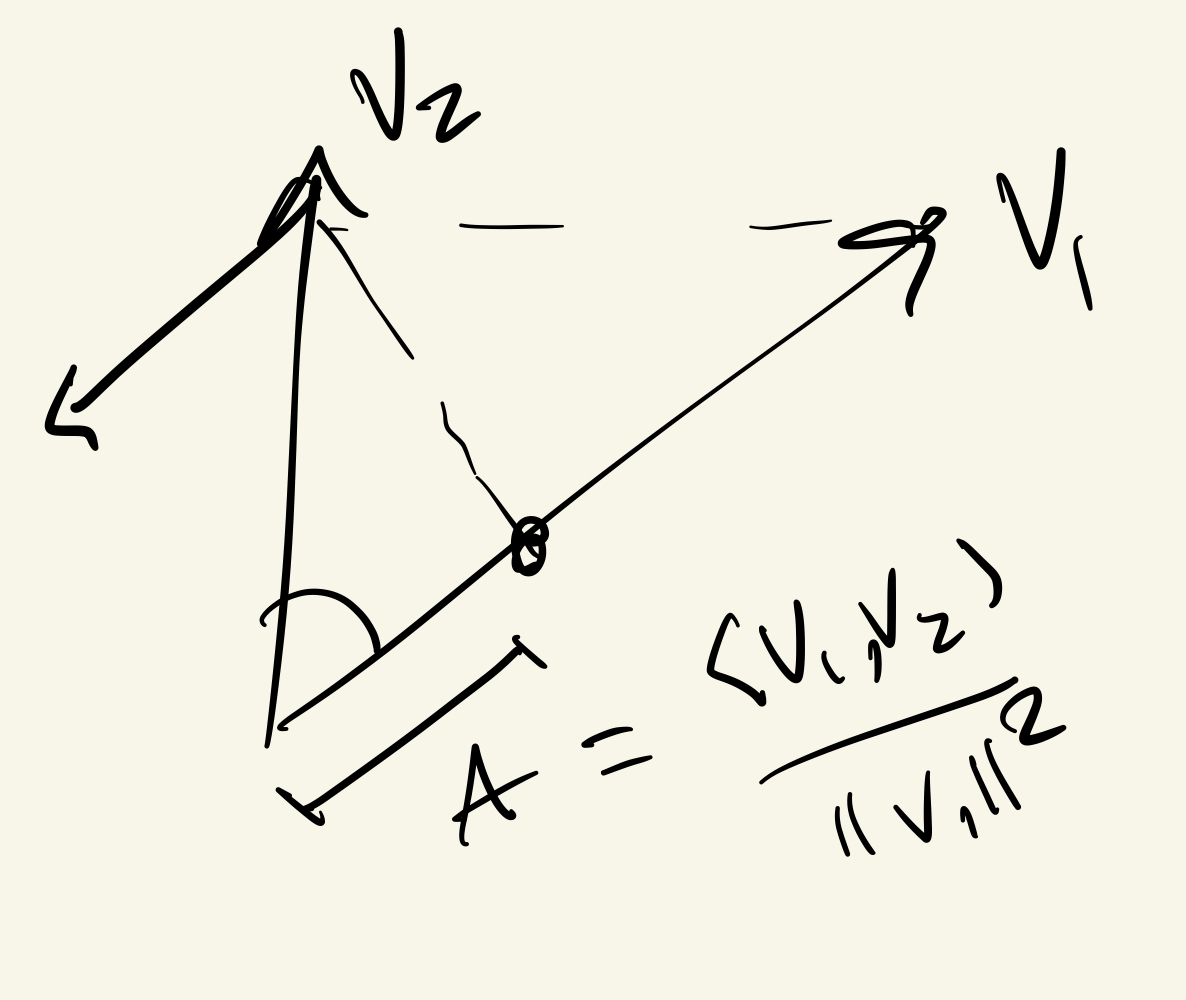
\includegraphics[width=0.3\textwidth]{fig1}
\end{figure}
The vector you are looking for is 
 \[v_2-Av_1=v_2-\frac{\left<v_2,v_1\right>}{\left<v_1,v_1\right>}v_1\]
 And most importantly never forget how to find \(A\):  ``dot product measures alignment---it's small when vector are almost perpendicular, and large when they are almost parallel---, to project a vector onto the other you need to know how much aligned they are, and normalize by the size of \(v_1\) because the size of \(v_1\) doesn't matter for projection".

\end{proof}

\begin{remark}\leavevmode
	O processo pode ser feito igualzinho para campos vetoriais: se \(X_1,\ldots,X_n\) é uma base local de campos, \(\exists !\) base ortonormal de campos \(\{e_i\}\). \textbf{Cuidado:} em geral, o colchete desses campos não é zero, i.e.  \([e_i,e_j] \neq 0\).
\end{remark}

\begin{prop}[Elemento de volume]\leavevmode
\(M^n\) variedade Riemanniana orientada  \(\implies\) \(\exists !\) \(\omega \in \Omega^{n}(M^n)\) tal que
\[\omega(\text{bon+} )=1\]
bon+=base ortonormal orientada.
\end{prop}

\begin{thing6}{Lembre}\leavevmode
Para duas top-forms, uma se expressa como a outra multiplicando pelo determinante da mudança de base.
\end{thing6}

\begin{proof}\leavevmode
Como \(M\) é orientada, sabemos que \(\exists  \sigma \in \Omega^{n}(M^n)\) positiva. Buscamos a função \(f\) tal que \(\omega=f\sigma\). Pega um ponto, bases coordenadas \(\{\partial_i\}\) e ortonormaliza para obter \(\{e_i\}\). Como queremos que
\[\omega(e_1,\ldots,e_n)\overset{\text{quero}}{=}1\overset{\text{quero}}{=}f|_{U}\sigma(e_1,\ldots,e_n)\]
só tem um jeito de definir \(f\):
\[f|_{U}=\sigma(e_1,\ldots,e_n).\]
E isso determina por completo \(f\) como uma função global suave, e portanto temos \(\omega\).
\end{proof}

\section{Aula 5}

\subsection{Todo fibrado vetorial pode ter métrica}

\begin{remark}[Todo fibrado vetorial pode ter métrica]\leavevmode
Se \(E\) é um fibrado vetorial sobre \(M\), então também podemos pegar seções de
 \[\begin{tikzcd}
\operatorname{B i l Si m}E\arrow[d]\\
M
\end{tikzcd}\]
qualquer um dessas seções é uma \textit{\textbf{métrica Riemanniana}} em \(E\):
\[\left<\cdot,\cdot\right>: \Gamma(E)\times \Gamma(E)\longrightarrow \mathcal{F}(M)\]
A prova de que tais métricas sempre existem é análoga à prova para o fibrado tangente.
\end{remark}

\subsection{Comprimento de curvas, distancia, \(M\) como espaço métrico}

Pegue \(\alpha:[a,b]\longrightarrow M\) diferenciável por partes, i.e. existe uma partição do intervalo \([a,b]\) em que \(\alpha\) é diferenciável em cada pedacinho. Isso significa que cada intervalsinho pode ser estendido um pouqinho para cada lado, de tal jeito que temos um intervalo aberto, que é uma variedade, então aí está definida a diferencial.

Então definimos
\[\ell(\alpha):=\int_a^b \|\alpha'(t)\|dt\]

\begin{remark}[A função comprimento não vê a parametrização da curva]\leavevmode
Se \(\varphi:I \to I'\), com \(\varphi' \geq 0\), então
\[\ell(\alpha \circ \varphi) = \ell(\alpha)\]
{\color{4}É só fórmula de mudança de variáveis, ver \cite{tud}, prop. 16.1.}
\iffalse\begin{thing4}{Proposition 16.1}[\cite{les}]\label{prop:16.1}\leavevmode
Suppose \(D\) and \(E\) are open domains of integration in \(\mathbb{R}^n\) (or \(\mathbb{H}^n\)) and \(G:\overline{D}\to \overline{E}\) is a smooth map that restricts to an orientation-preserving or orientation-reversing diffeomorphism from \(D\) to \(E\). If \(\omega\) is an \(n\)-form on \(\overline{E}\), then
\[\int_D G^*\omega=\begin{cases}
	\int_E \omega\qquad &\text{ if \(G\) is orientation-preserving}  \\
	-\int_E \omega\qquad &\text{ if \(G\) is orientation-reversing} 
\end{cases}\]
\end{thing4}\fi
\end{remark}

Como \(M^n\) é conexa (todas as nossas coisas são conexas) quaisquer dois pontos \(p,q \in M\) estão ligados por uma curva, então podemos definir
\[d(p,q):= \operatorname{inf}\{ \ell (\alpha),\alpha:[a,b] \to M \text{ d.p.p., }\alpha(a)=p,\alpha(b)=q \}\]

Para ver que \(d\) é simétrica pode usar a mesma curva em sentido contrário. Para ver desigualdad triangular usamos diferenciabilidade por partes e definição de ínfimo (tinha um \(\varepsilon\)).

Para ver que \(d(p,p)=0\) pegue uma carta  \((x,U)\) em \(p \in M\). Existe \(B_r(x(p)) \subset x(U)\) cujo fecho queda dentro de \(x (U)\). Então \(\overline{x^{-1}(B)} \subset U\) compacto.

Os autovalores da matrix \((g)_{ij}\) são sempre positivos porque a métrica é positiva definida. Então como estamos num compacto existe uma cota inferior. Fica que existe \(\delta>0\) tal que \(\forall  v \in T(\times^{-1}(B)\)


A ver entonces aparece una \(\delta\) que es la cota de los autovalores de la métrica. {\color{7}Checar} ese asunto de que los autovalores son positivos. El chiste es que ahí la métrica en el espacio tangente se vuelve equivalente a la métrica aplicando la diferencial (foto)

Em conclusão, \((M^n, d)\) é um espaço metrico.

\begin{exercise}\leavevmode
Mostre que a topologia métrica coincide com a topologia métrica. \textbf{Hint}. usar a desigualdade da foto, e meter uma bola dentro de outra.)
\end{exercise}

Segue do exercício 	que \(d\) é contínua.

\begin{remark}\leavevmode
Em variedades semi-Riemannianas não podemos fazer essa construção!
\end{remark}

\subsection{Conexão afim}

Pegue \(Z \in \mathfrak{X}(\mathbb{R}^n)\), \(Z=(z_1,\ldots,z_n)\), \(z_i \in \mathcal{F}(\mathbb{R}^n)\). Podemos derivar--- nomas deriva coordenada a coordenada {\color{7}(pegando uma  base!)}:

*Checar derivada covariante em \(\mathbb{R}^n\) com \cite{tud}*

\begin{defn}\leavevmode
Uma \textit{\textbf{conexão}} ou \textit{\textbf{derivada covariante}} em \(M\) é um operador \(\mathbb{R}\)-bilinear
\begin{align*}
	\nabla: \mathfrak{X}(M) \times \mathfrak{X}(M) &\longrightarrow \mathfrak{X}(M) \\
	(Y,Z) &\longmapsto \nabla_YZ
\end{align*}
que é tensorial em \(Y\) e uma derivação em \(Z\), ou seja,
\[\nabla_Y(hZ)=Y(h)Z+h\nabla_YZ\qquad  \forall  Y,Z \forall h \in \mathcal{F}(M)\]
\end{defn}

\begin{remark}[dani]\leavevmode
A derivada covariante não é um tensor; não pode ser vista como a seção de um fibrado sobre \(M\). Em câmbio, ela é um operador entre certos espaços de seções. Acho que isso vai ser assim para todo operador diferencial com que a gente vai trabalhar…
\end{remark}

Olhando o exemplo de \(\mathbb{R}^n\), os espaços vetoriais tem uma conexão canônica.

O que falta a uma conexão para ser um tensor e uma coisa que não depende de D. Então a diferencia de duas derivações é um tensor! Por isso se chama conexao afim.

\begin{defn}\leavevmode
Uma \textit{\textbf{conexão}} ou \textit{\textbf{derivada covariante}} no fibrado vetorial \(E\) é um operador \(\mathbb{R}\)-bilinear
\begin{align*}
	\nabla: \mathfrak{X}(M) \times \Gamma(E) &\longrightarrow \Gamma(E) \\
	(Y,Z) &\longmapsto \nabla_YZ
\end{align*}
que é tensorial em \(Y\) e uma derivação em \(Z\), ou seja,
\[\nabla_Y(hZ)=Y(h)Z+h\nabla_YZ\qquad  \forall  Y,Z \forall h \in \mathcal{F}(M)\]
\end{defn}

A diferencia fundamental con a conexão em \(\mathbb{R}^n\) é que essa é canônica. Em geral não!

Note essa propriedade aqui da conexão afim real:
\begin{align*}
Y\left<Z,Z'\right>&=\sum Y(z_i)z_i'+\sum z_i Y(z_i')\\
&=\left<D_YZ,Z'\right>+\left<Z,D_YZ'\right>
\end{align*}
Essa é uma propriedade bacana. Você pode conferir, só escrevendo, que
\[D_YZ-D_ZY=[Y,Z]\]
Aqui tem que fazer a conta (``o que falha para \(Y\) em  \(D_YZ\),  é o que falha para \(Y\) em \([Y,Z]\)"), mas fica que
\[D_YZ-D_ZY-[Y,Z]:=T(Y,Z)\]
\textbf{é tensorial}. Esse tensor se chama \textit{\textbf{torsão}}.

No caso de \(\mathbb{R}^n\), fica que isso é zero. Essa conexão é bem especial.

Agora vamos fazer algumas observações. A primeira é uma brincadeira que fica ``pela tensorialidade":

Seja \(\nabla\) uma conexão em \(M\) (ou \(E\)), então escrevemos para \(p \in M, v \in T_pM\),
\[\nabla_v Y = (\nabla_X Y)(p)\]
Em particular, \(f :N \to M\), \((\nabla_{X \circ f}Y)=(\nabla_XY)\circ f\in \mathfrak{X}_f\), ou seja podemos obter um campo \textit{ao longo de \(f\)}…  
\begin{prop}\leavevmode
\(\nabla\) é um \textit{\textbf{operador local}}, i.e. \(\forall  X,X' \in \mathfrak{X}(M), Y,Y' \in \mathfrak{X}(M)\) e \(U \subset M\) aberto, se
\[X|_{ U}=X'|_{U},\qquad Y|_{U}=Y|_{U}\]
então
\[(\nabla_XY)|_{U}=(\nabla_{X'}Y')|_{U}\]
\end{prop}
\begin{thing7}{Tentação}\leavevmode
Defina \(Z:=Y-Y'\)  então como \(Y|_{ U}=Y'|_{U}\), \(Z\) é constante e \(\nabla Z=0\). Porém, que \(Y\) coincida com \(Y'\) em \(U\) não significa que \(Z\) é zero como campo \textit{em toda \(M\)}. 
\end{thing7}
\begin{proof}[Demostração beleza de \cite{milnorch}, p. 294 app. C]\leavevmode
Defina \(Z=Y-Y' \in \mathfrak{X}(M)\). Ele não tem por que ser zero; só sabemos que é zero em \(U\). Queremos ver que \(\nabla_XZ\) também é zero em \(U\). Então pega um ponto \(p \in U\) e uma função \(\rho\) que vale \(1\) perto de \(p\) e zero fora de \(U\).

{\color{7}Se tem muita vontade de pensar em como funciona isso faça assim. Pegue um aberto \(V \subset U\) tal que \(\overline{V}\subset U\). Pegue uma partição da unidade \(\{\rho,\lambda\}\) subordinada à coberta \(\{U,M\setminus \overline{V}\}\). Fica que
\begin{align*}
\begin{aligned}
\operatorname{supp}\rho &  \subset U\\
\operatorname{supp}\lambda &  \subset M\setminus \overline{V}\\
\rho+\lambda & \equiv 1
\end{aligned}
\quad \implies \rho |_{(\operatorname{supp}\lambda)^c}\equiv 1 \implies \rho |_{V}\equiv 1
\end{align*}}
O importante é que
\[\rho Z \equiv 0 \in \mathfrak{X}(M)\]
é outra cara do campo vetorial zero. Então obviamente
\[0=\nabla_X(\rho Z)=X(\rho)Z+\rho \nabla_XZ\]
E agora avalia em \(p\)! Fica que \((\nabla_XZ)_p=0\) \(\forall  p \in U\).
\end{proof}
\iffalse\begin{proof}\leavevmode
Realmente é a tentação feita bem. Defina \(Z\) \textit{con todas las de la ley} como sendo um campo vetorial em \(U\) dado por
\[Z:=Y|_{U}-Y'|_{U}\in \mathfrak{X}(U)\]
Queremos ver que \((\nabla_XZ)_p=0\) para qualquer ponto \(p \in U\).

O trabalho e estender \(Z\) a um campo em todo \(M\). Como é que é? Pega uma coberta \(\{U,M\setminus \overline{V}\}\) onde \(V \subset \overline{V}\subset U\) é pseudo(quase,para?)compacto (fecho compacto) e uma partição da unidade \(\{\rho,\lambda\}\) subordinada. Isso diz que
\begin{align*}
\begin{aligned}
\operatorname{supp}\rho &  \subset U\\
\operatorname{supp}\lambda &  \subset M\setminus \overline{V}\\
\rho+\lambda & \equiv 1
\end{aligned}
\quad \implies \rho |_{(\operatorname{supp}\lambda)^c}\equiv 1 \implies \rho |_{V}\equiv 1
\end{align*}
Então 
\[\rho Z \in \mathfrak{X}(M)\]
e posso derivá-lo:
\[\nabla_X\rho Z=\nabla_X 0=0\]
Em \(V\), isso diz que
\[\nabla_{X|_{V}}(Y-Y')|_{V}=0\]
E parece que acabei mas isso não é como eu queria: eu queria em \(U\).

Em \(U\) tem lugares onde \(\rho \neq 1\). Pero eso sí:  \(\rho|_{U}\) é uma função em \(U\) e \(Z\) é um campo vetorial em \(U\) (porque \(Z\) só existe como elemento de \(\mathfrak{X}(U)\)!). Então tenho Leibniz perto de qualquer ponto dentro de \(U\):
\begin{align*}
0=\nabla_{X|_{U}}\rho Z&=\underbrace{X|_{U}(\rho)
}_{\substack{\text{pode não}  \\ \text{ser 0} } }\underbrace{Z}_{=0}+\rho|_{U} \nabla_{X|_{U}} Z
\end{align*}


	Pegue \(p \in U\), \(p \in V \subset \overline{V}\subset U\).


	Antes de chegar a que é zero em \(p\) vimos que era zero em todo \(V\)… y antes acho que tinha escrito que era zero em \(U\)…
\end{proof}\fi

\begin{coro}\leavevmode
Dada uma conexão \(\nabla\) numa variedade \(M\), existe uma única conexão \(\nabla^U\) em \(U\) que faz
\[\nabla^U_{X|_{U}}Y|_{U}=(\nabla_XY)|_{U}\]
\end{coro}
\begin{remark}\leavevmode
Note que  nem todo campo em \(U\) pode ser escrito assim: pode ter um campo que faz coisas estranhas em \(\partial U\) y acaba que não se estende.
\end{remark}

Beleza

Agora pegue \((x,U)\) carta em  \((M,\nabla)\). Sabemos que debem existir as seguintes funções:
\[\nabla_{\partial_i}^U\partial_j:=\sum \Gamma_{ij}^k \partial_k\]
que se chamam \textit{\textbf{símbolos de Christoffel}} de \(\nabla\) na carta \((x,U)\).

Agora vamos ver que esses símbolos determinam \(\nabla\) *se echa la cuenta del O'Neill*
\begin{thing4}{Proposition 3.13}[\cite{oni}]\label{prop:3.13}\leavevmode
For a coordinate system \(x^1,\ldots,x^n\) on \(U\),
\begin{enumerate}
	\item {\color{7}Essa aqui ele provou, é só escrever:}\[D_{\partial_i}\left(\sum W^j\partial_j\right) =\sum_{k}\left(\frac{\partial W^k}{\partial x^i}+\sum_{j}\Gamma_{ij}^kW^j\right) \partial_k.\] 
	\item {\color{7}Essa aqui ainda não usamos:} \[\Gamma_{ij}^k=\frac{1}{2}\sum_{m}g^{km}\left(\frac{\partial g_{jm}}{\partial x^i}+\frac{\partial g_{im}}{\partial x^k}-\frac{\partial g_{ij}}{\partial x^m}\right) \]
	
\end{enumerate}
\end{thing4}
\[\text{*contas*} \]

E no final note que pode restringir tudo beleza então fica que ``os símbolos de Christoffel determinam a conexão".

Bom agora, como se vê isso em fibrados? Pegue
\[\begin{tikzcd}
E^k\arrow[d]\\
M
\end{tikzcd}\]
uma carta trivializante \((\varphi, \pi^{-1}(U))\), \(\{\xi_1,\ldots,\xi_n\}\) base de \(\Gamma(\pi^{-1}(U))\). Pegue \(X \in \mathfrak{X}(M)\), \(\xi \in \Gamma(E)\), com \(\xi=\sum \lambda_i\xi_i\), então (as contas são todas iguais…)
\[(\nabla_X \xi)|_{U}=\nabla_{\sum x_i \partial_i}\sum \lambda_j \xi_j\]
e no final fica que
\[\nabla_{\partial_i}\xi_j=\sum_k\Gamma_{ij}^k \xi_k\]

Lo que sigue es importantísimo (existe una única sección que le hace así…): pegue um fibrado afim
\[\begin{tikzcd}
f^*E\arrow[d]&(E,\nabla)\arrow[d,"\pi"]\\
N\arrow[r,"f",swap]&M
\end{tikzcd}\]
Para \(X \in \mathfrak{X}(N)\) e \(\xi \in \Gamma(E)\) podemos construir uma seção a longo de \(f\), namely \(\xi \circ f \in \Gamma(f^* E)\). E claro também temos \(f_*X \in \mathfrak{X}_f\). E também
\[\nabla_{f_*X}\xi\]
é uma seção desse fibrado pullback.

\begin{prop}\leavevmode
Para todo fibrado sobre \(M\) e função \(f\), existe uma única conexão \(\nabla^f\) tal que
\[\nabla_X^f(\xi \circ f)=\nabla_{f_*X}\xi \in \Gamma(f^*E)\]
{\color{2}Acho que tá errado: na entrada  ``\(X\)" \textbf{não} podemos ter seções de \(f^*E\), i.e. esse \(f_*X\) em baixo tá errado.}
\end{prop}
\begin{remark}\leavevmode
Nem toda seção de \(f^*E\) se escreve como \(\xi \circ f\). Pense em \(f\) constante. Então as seções \(\xi \circ f\) são seções constantes (porque \(f^*E\) é o fibrado trivial, faz sentido dizer ``seção constante"). Mas nem toda seção do fibrado trivial é constante…

Mas localmente sim {\color{2}(isso é o lance! A prova é: pega uma trivialização local de \(E\), ali tem um marco \(\{\xi_i\}\), pega um aberto coordenado \(V \subset N\) t.q. \(f(V)\subset U\), e vai ter que as seções ao longo de \(f\), cujos vetores estão em \(\pi^{-1}(U)\subset E\), são combinação linear das \(\xi_i\), então por definição de pullback bandle as seções ao longo de \(f\) em \(V\) são combinação linear de \(\xi_i \circ f\).)}
\end{remark}

\begin{proof}\leavevmode
Seja \(p \in N\), \(U \subset M\) aberto, \((\varphi,U)\) carta trivializante de \(E\) em \(f(p)\). Primeiro suponha que essa coisa existe para ver que cara tem. Vamos definir para \(\lambda \in \Gamma(f^*E)\) e \(X \in \mathfrak{X}(N)\)
\[(\nabla_X^f \lambda)|_{U}=\nabla_{X|_{U}}^f \lambda|_{U}\]
Queremos ver qual é o valor em \(p \in V \subset N\), \(f(V) \subset U \subset M\). Em \(U\) temos \(\{\xi_1,\ldots,\xi_k\}\) base de seções de \(\pi^{-1}(U)\).

Seja \(q \in V\). Então
\[\lambda(q)=\sum\lambda_i(q) \xi_i(f(q))\]
E que ficou?
\[\lambda|_{V}=\sum\lambda_i{\color{7}|_{V}} {\color{7}(}\xi_i \circ f{\color{7})|_{V}}\]
Usando a definição de \(\nabla\) como derivação em \(Y\)… podemos provar unicidade local. {\color{2}Como estamos supondo que \(\nabla^f\) existe, deve ser um operador local, i.e. existe} 
\[\nabla^f \rightsquigarrow  (\nabla^f)^V,\]
{\color{2}mas ainda, estamos supondo que \(\nabla^f\) é boa nas seções da forma \(\xi_i \circ f\) }:
\begin{align*}
\nabla_{X|_{V}}^f(\lambda|_{V})&=\sum\nabla_{X|_{V}}\lambda|_{V}(\xi_i \circ f)|_{V}\overset{\operatorname{hip}}{=}\sum X(\lambda_i)(\xi_i \circ f)+\lambda_i\nabla_{f_*X}\xi_i
\end{align*}
Ou seja, isso define uma unicamente uma conexão em \((f|_{V})^*(\pi^{-1}(U))\).

Mas, como a conexão é um operador local, isso prova também unicidade global. 

Para ver existência, pois é, como sabemos que é única localmente e coincide nas interseções, existe.

Definimos \(\nabla^f\) localmente, i.e. como uma conexão em \((f|_{V})^*(\pi^{-1}(U))\).

\begin{exercise}\leavevmode
Verifique que satisfaze as propriedades de conexão (\(\mathbb{R}\)-linear, tensorial e derivação).
\end{exercise}
\begin{proof}[Solução]\leavevmode
\begin{enumerate}
\item \textbf{(\( \mathbb{R}\)-linear em \(\lambda\).)} Acho que o mais importante é o setting: pegamos \(U\subset M\), \(V \subset N\) com \(f(V)\subset U\). Pegue \(\alpha \in \mathbb{R}\) e \(\lambda,\mu \in \Gamma(f^*E)\). E dizemos bom, já construímos \(\nabla^f\) como operador global, então podemos restringi-lo a \(V\):
	\[\nabla_X^f(\alpha \lambda+\mu)\Big|_{V}\overset{\operatorname{def}}{=}\nabla_{X|_{V}}^f(\alpha \lambda +\mu)|_{V}\]
E dizemos bom, de fato ele foi definido como sendo o cara que localmente é o que queremos, então naturalmente, em \(V\),
\[\nabla^f_{X|_{V}}(\alpha\lambda+\mu)|_{V}=\alpha\nabla^f_{X|_{V}}\lambda|_{V}+\nabla^f_{X|_{V}}\mu|_{V}\]
E dizemos que como é único em \(V\), e está bem definido localmente, essa igualdade é verdade globalmente.
\item \textbf{(Leibniz em \(\lambda\).)} Pegue \(g \in \mathcal{F}(N)\), \(\lambda\in\Gamma(f^*E)\), os conjuntinhos que faz tudo funcionar localmente e diga:
	\begin{align*}
	\nabla^f_X(g\lambda)\Big|_{V}&=\nabla^f_{X|_{V}}\Big((g\lambda)|_{V}\Big)=X|_{V}(g|_{V}) \lambda|_{V}+g|_{V}\nabla^f_{X|_{V}}\lambda|_{V}
	\end{align*}
\item \textbf{(\(\mathcal{F}(N)\)-linear em \(X\).)} Pegue \(g \in \mathcal{F}(N)\), \(X,Y \in \mathfrak{X}(N)\) e \(\lambda \in \Gamma(f^*E)\). Localmente,
	\begin{align*}
	\nabla^f_{gX+Y}\lambda\Big|_{V}&\overset{\operatorname{def}}{=}\nabla^f_{(gX+Y)|_{V}}\lambda |_{V}=g|_{V}\nabla^f_{X|_{V}}\lambda|_{V}+\nabla^f_{Y|_{V}}\lambda|_{V}=\Big(g\nabla^f_X\lambda+\nabla^f_Y\lambda\Big)\Big|_{V}
	\end{align*}
	todo mundo cola e pronto.
\end{enumerate}
\end{proof}
\end{proof}

Sendo assim que demostramos a primeira propriedade mágica do pullack: ele puxa conexões. Também podemos puxar a métrica.

\begin{example}[Isto é equivalente à localidade da conexão]\leavevmode
\[\begin{tikzcd}
	\pi^{-1}(U)=\text{inc}^* (E)\arrow[d]&E\arrow[d,"\pi"]\\
	U\arrow[r,hook,"\text{inc}"]&M
\end{tikzcd}\]
\end{example}
\begin{remark}\leavevmode
*Comentários sobre o caso quando \(f\) é uma curva \(\alpha:I \to M\),
\[\begin{tikzcd}
	(\alpha ^* (E),\nabla^\alpha)\arrow[d]& (E,\nabla)\arrow[d,"\pi"]\\I\arrow[r,"\alpha",swap]&M
\end{tikzcd}\]
\end{remark}

\begin{thing8}{O que aconteceu}\leavevmode
Mostramos que a derivada covariante é um operador local e isso permite puxar a conexão para o pullback bundle.
\end{thing8}

\begin{thing9}{Miração}\leavevmode
Vamos mostrar que a curvatura é um operador local e vamos puxá-la.
\end{thing9}

\begin{thing8}{Dúvidas para consultar}\leavevmode
\begin{itemize}
\item Pergunta sobre exercício de métrica bi-invriante em grupo de Lie compacto.
\item Exercício de pullback bandle.
\item Que onda con eso del espacio métrico y que la distancia de un punto a sí mismo es cero.
\end{itemize}
\end{thing8}


\section{Aula 6}

\subsection{Transporte paralelo.}

\begin{remark}[Pullback connection for curves]\leavevmode
É para esclarecer o problema com a notação
\[\nabla_{\alpha'}\alpha'\]
quando \(\alpha:I \subset \mathbb{R} \to M\). Normalmente que é o que fazemos? Pegamos uma extensão local \(Y\) de \(\alpha'\), o último sendo um campo vetorial \textit{ao longo de \(\alpha\)} (o que isso signifique), e calculamos a derivada covariante \(\nabla_YY\) sobre a curva \(\alpha\). Ou seja \((\nabla_YY)\circ\alpha\). Pero a la mera hora:
\[(\nabla_YY)\circ \alpha=\nabla_{Y\circ\alpha}Y=\nabla_{\alpha_*\frac{d}{dt}}Y=\nabla^\alpha_{\frac{d}{dt}}Y \circ \alpha=\nabla^\alpha_{\frac{d}{dt}}\alpha'\]
E é isso:
\[\underbrace{\nabla_{\alpha'}\alpha'}_{\text{não} }=\underbrace{\nabla^\alpha_{\frac{d}{dt}}\alpha'}_{\text{que bom} }\]
\end{remark}

\begin{exercise}\leavevmode
\begin{enumerate}
\item Dar sentido e provar
	\[g^*(f^*(E))=(f\circ g)^*(E)\]
	\[(\nabla^f)^g=\nabla^{f \circ g}\]
\item \(p \in M\), \(i :N \hookrightarrow  M\times N\) inclusão, \(\tilde{f}:M\times N\to (\tilde{M},\nabla)\). Se \(X \overset{i}{\sim}\tilde{X}\), \(Y \overset{i}{\sim}\tilde{Y}\),
\[(\nabla_{\tilde{X}}^{\tilde{f}}\tilde{f}_*\tilde{Y})\circ i=(\nabla_X^f f_*Y)\]
onde \(f:=\tilde{f} \circ i\). \textbf{Ideia:} é como fixar todas as variávis e derivar a função de uma  variável que fica (para calcular a derivada parcial).
\item \(f:M \to (\tilde{M},\nabla)\),
	\[\nabla^f_X(f_*Y)=f^* (\nabla_{\tilde{X}}\tilde{Y}\qquad  \forall  f:X \to \tilde{X}, f:Y \to \tilde{Y}\]
\end{enumerate}
\end{exercise}
\begin{proof}[Solução]\leavevmode
\begin{enumerate}
\item Um elemento \((q,v)\in (f\circ g)^*E\) satisfaz que \((f(g((q))=\pi(v)\). Isso diz que \((g(q),v)\) é um elemento de \(f^*E\). De fato, isso diz que \((q,v)\) é um elemento de \(g^*f^*E\). Reciprocamente, um elemento \((q,v)\in g^*f^*E\) satisfaz que \(g(q)=\pi_f(v)\). Então \(v \in E\) e \(f(g(q))=\pi(v)\), é isso é estar em \((f\circ g)^*E\).
\end{enumerate}
\end{proof}
Agora sim, considere esse caso particular:
\[\begin{tikzcd}
	(\alpha^*(TM),\nabla^\alpha)\arrow[d]&(TM,\nabla)\arrow[d]\\
	I\subset\mathbb{R}\arrow[r,swap,"\alpha"]&M
\end{tikzcd}\]
Então para \(V \in \mathfrak{X}_\alpha\) definimos
\[\nabla_{\frac{d}{dt}}^\alpha V:=V'\in \mathfrak{X}_\alpha\]
Agora pegue uma vizinhança coordenada \((x,U)\) de \(M\) em \(p:=\alpha(0)\), de modo que exista \(\varepsilon>0\) tal que \(\alpha\)

Derivar \(V\) ao longo de \(\alpha\), calcular.

Fica uma derivação de primeira ordem em \(V\)…

\begin{remark}\leavevmode
\(V'=0\) \(\iff\), localmente, todas as funções coordenadas são zero. Sendo um sistema de primeira ordem, temos existência e uncidade das soluções, i.e.
\[\forall  v \in T_p M\; \exists ! V_v \in \mathfrak{X}_\alpha \text{ t.q. } V'=0\text{ e } V_v(p)=v.\]
\end{remark}

Os \textit{\textbf{campos paralelos ao longo de \(\alpha\)}} são
\[\mathfrak{X}''_\alpha:=\{V \in \mathfrak{X}_\alpha:V'=0\}\]
fica isomorfo ao espaço tangente em \(p\), i.e.
\[\mathfrak{X}''_\alpha \cong T_pM\]
\begin{remark}\leavevmode
Isso depende de \(\alpha\), claro, se tu pega um campo em \(M\) que é paralelo a \(\alpha\), pode não ser paralelo ao longo de outra curva. Considere a seguinte situação: que em todo ponto tenha uma base das seções que \textit{são paralelas ao longo de qualquer curva}. Então tu tá em \(\mathbb{R}^n\). Vamos demostrar isso.
\end{remark}

Tem mais: essa construção aqui nos permite ``conectar os espaços tangentes ao longo de curvas que ligam esses pontos". Claro, pega um vector em \(p\), pega uma curva que liga \(p\) a \(q\), e defina o \textit{\textbf{transporte paralelo dele}} como o vector em \(q\) do campo paralelo ao longo de  \(\alpha\). Esse mapa se chama
\[P_{ab}^\alpha:T_pM \to T_q M\]
E isso \textit{super} depende de \(\alpha\). Tanto assim que se não depende de \(\alpha\) é porque estamos em \(\mathbb{R}^n\).

\subsection{Derivada covariante de qualquer tensor. Métrica Compatível.}

Temos um operador
\[\nabla:\mathfrak{X}(X) \times \mathfrak{X}(X) \longrightarrow \mathfrak{X}(X)\]
mas pode fixar \(X \in \mathfrak{X}(X)\) para obter:
\[\nabla_X:\mathfrak{X}(X)\longrightarrow \mathfrak{X}(X)\]
Agora pense numa função \(f \in \mathcal{F}(M)\). Então temos um operador
\begin{align*}
	\nabla_X: \mathcal{F}(M) &\longrightarrow \mathcal{F}(M) \\
	f &\longmapsto \nabla_Xf=Xf
\end{align*}
Agora pense num \((2,0)\)-tensor \(T\). Então queremos ter
\begin{align*}
	\nabla_X: T^{2,0}(M) &\longrightarrow T^{2,0}(M) \\
	T &\longmapsto \nabla_X T
\end{align*}
Mas como definimos esse cara \(\nabla_X T\)? Bom pegue dois campos \(Y,Z \in \mathfrak{X}(M)\) e faça
\[(\nabla_X T)(Y,Z):=X(T(Y,Z))\]
que faz sentido porque, lembre, lembre sempre, que um tensor é uma seção do fibrado no sé qué produto tensorial das seções e o dual no sé que, e isso é a mesma coisa que um mapa \(\mathcal{F}(M)\) multilinear, nesse caso, \(\mathfrak{X}(M)\times \mathfrak{X}(M) \to \mathcal{F}(M)\). Então fica que \(T(Y,Z) \in \mathcal{F}(M)\) e por isso posso avaliá-lo em \(X\). Mas tem um problema: \(X(T(Y,Z))\) não é tensorial porque é um operador diferencial, i.e. ele é Leibniz, olha:
\[X(T(fY,Z))\overset{T \text{ tensor} }{=}X(f(T(Y,Z))\overset{X \text{ op. dif.} }{=}Xf T(Y,Z)+f X(T(Y,Z))\]
e isso não é como eu queria. Eu queria
\[\underbrace{(\nabla_X T)}_{\text{tensor} }(fY,Z)=f (\nabla_X T)(Y,Z)\overset{\operatorname{def}}{=}fX(T(Y,Z))\]
Então fica que sobra esse termo \(f(\nabla_X T)(Y,Z)\). Então resulta (milagre?) que simplesmente restando esse termo o negocio fica tensorial e por fim já entendi por que
\[(\nabla_X T)(Y,Z)\underbrace{:=}_{\text{que bom}}X(T(Y,Z))-Xf T(Y,Z).\]
E isso generaliza como tu já sabe. Fica que pode derivar qualquer tensor em \(T^{\bullet,\bullet}(M)\) para obter um tensor do mesmo tipo.

Um tensor cuja derivada covariante é zero é chamado \textit{\textbf{paralelo}}. Já tínhamos notado que a métrica euclidiana é paralelo respeito a conexão natural. Isso se chama de \textit{\textbf{métrica compatível}}.

\begin{thing8}{Milagre}\leavevmode
Se \(M\) é uma variedade (pseudo-)Riemanniana, existe uma única conexão \(\nabla\) em \(TM\) que é simétrica (= torsão é zero) e compatível com a métrica. Essa conexão se chama \textit{\textbf{conexão de Levi-Civita}}.
\end{thing8}

\begin{remark}\leavevmode
Isso é um motivo para trabalhar com produtos internos em lugar de normas; não tem milagre para norma.
\end{remark}

\begin{proof}[Prova do milagre]\leavevmode
Pegue treis campos \(X,Y,Z \in \mathfrak{X}(M)\) e faça a seguinte brincadeira
\[Z \left<Y,Z\right>+Y\left<X,Z\right>-Z\left<X,Y\right>\]
Então compute, some o término que falta, tire pra um lado tudo que tem \(\nabla\), e note que isso mostra unicidade. Se existe, é única.

\begin{exercise}\leavevmode
Agora defina um operador \(L\) como satisfazendo essa fórmula (se chama \textit{\textbf{fórmula de Koszul}}), e prove que essa \(L\) é uma conexão simétrica e métrica.\end{exercise}
\end{proof}

\begin{thing7}{Conta em coordenadas}\leavevmode
Agora usamos Koszul para ver que
\[2\left<\nabla_{\partial_i}\partial_j,\partial_k\right>=\frac{\partial g_{ij}}{\partial x_i}+\frac{\partial g_{ik}}{\partial x_j}-\frac{\partial g_{ij}}{\partial x_k}\]
Dai expande o colchete do lado esquerdo obtendo os símbolos de Christoffel, e dai multiplica os dois lados pela matrix inversa da métrica.
No final fica que
\[2\Gamma_{ij}^\ell=\sum_k g^{k\ell}\frac{\partial g_{ij}}{\partial x_i}+\frac{\partial g_{ik}}{\partial x_j}-\frac{\partial g_{ij}}{\partial x_k}\]
Ou seja, a conexão está determinada pelos símbolos de Christoffel. Que estão determinados pela métrica. Então fica que a conexão é uma função da métrica e das derivadas parciais da métrica, i.e.
\[\nabla=\mathcal{F}\Big(\left<\cdot,\cdot\right>,\partial \left<\cdot,\cdot\right>\Big)\]
\end{thing7}

\begin{coro}\leavevmode
Como a métrica não muda em \(\mathbb{R}^n\), os símbolos de Christoffel se anulam.
\end{coro}

\begin{exercise}\leavevmode
Uma conexão é compatível com uma métrica \(\iff\) 
\begin{align*}
\forall \alpha, \forall V,W \in \mathfrak{X}_\alpha,\qquad \left<V,W\right>'&=\left<V',W\right>+\left<V,W'\right>\\
&\iff\\
\forall \alpha, \forall V,W \in \mathfrak{X}''_\alpha,\qquad \left<V,W\right>&=\operatorname{cte}\\
&\iff\\
\forall \alpha, \forall t,s,\qquad  P_{t,s}^\alpha &\text{ são isometrias} \\
&\iff\\
\nabla \left<\cdot,\cdot\right>&=0
\end{align*}
\end{exercise}

\begin{exercise}\leavevmode
\((G,\left<\cdot,\cdot\right>)\) com \(\left<\cdot,\cdot\right>\) bi-invariante. Então a conexão de Levi-Civita em \(G\) satisfaz (e, caso \(\left<\cdot,\cdot\right>\) for simétrica, é caracterizada por)
\[\forall X \in \mathfrak{g}=\{\text{campo invariante à esquerda}\}, \qquad \qquad \nabla_XX=0\]
\textbf{Hint.} Use Koszul e o primeiro exercício das notas (quais notas? As notas de Florit).
\end{exercise}

\begin{remark}\leavevmode
Note que para puxar a métrica para o fibrado pullback não precisamos provar, porque os vetores são exatamente vetores no fibrado original.
\end{remark}

\begin{lemma}[de simetria e compatibilidade]\leavevmode
	(Conexao métrica puxa a conexão métrica, livre de torsão a livre de torsão.) Seja \(N\) variedade, \(f:N \to (M,TM,\left<\cdot,\cdot\right>,\nabla)\). Então
	\begin{enumerate}
	\item \(\nabla^f\) é \textbf{simétrica} , i.e.
		\[\forall X,Y \in \mathfrak{X}(N),\qquad \nabla^f_X f_*Y-\nabla^f_Y f_*X-f_*[X,Y]=0\]
	\item \(\nabla^f\) é compatível com \(\left<\cdot,\cdot\right> \circ f\)
	\end{enumerate}
	\begin{exercise}\leavevmode
		\(T_{\nabla f}=f^* T_\nabla\) 
	\end{exercise}
\end{lemma}

\begin{example}\leavevmode
Agora considere o caso de uma imersão isométrica. Fica que \textit{a parte tangente} do pullback da conexão (e da métrica também mas isso é obvio pq pedimos imersão isométrica) é a conexão de Levi-Civita.
\end{example}

\clearpage\bibliography{bib.bib}\end{document}
